\chapter{相关理论概述}

强化学习用于解决序贯决策问题,即需要连续不断地做出决策才能实现最终的目标,而序贯决策问题一般可以使用马尔科夫决策过程(Markov Decision Process, MDP)进行描述\citep{强化学习中离策略算法的分析和研究}。在利用MDP将序贯决策问题形式化后,又可以使用基于模型的动态规划方法和基于无模型的强化学习方法来求解该问题。特别地,在强化学习方法中,对于状态和行为空间较大的问题,往往采用值函数逼近的方法进行解决。本章会依次对上述内容进行介绍。

\section{强化学习概述}
强化学习是机器学习(Machine Learning, ML)的重要组成部分,它是从控制工程、心理学和运筹学等众多学科交叉发展而来的。强化学习最早可以追溯到十九世纪九十年代的巴普洛夫条件反射实验,但是,直到二十世纪九十年代才被重视起来,并随着相关理论和技术的不断完善,目前已经成为人工智能领域最火热的研究方向,广泛应用于机器人控制、无人驾驶和游戏等领域\citep{2016连续空间强化学习研究}。

强化学习主要用于解决序贯决策问题,所谓决策,是指面对特定的状态,采取什么样的行为,才能使得回报最大化;所谓序贯,是指需要连续不断地做出决策。所以,强化学习通过智能体(Agent)与环境持续地进行交互,并以最大化未来累积奖赏作为优化目标,从环境反馈的信息中不断学习,属于一种交互式的学习方法。具体交互过程如图$\ref{fig:强化学习过程}$所示:
% \begin{figure}[htbp]
% \centering
% 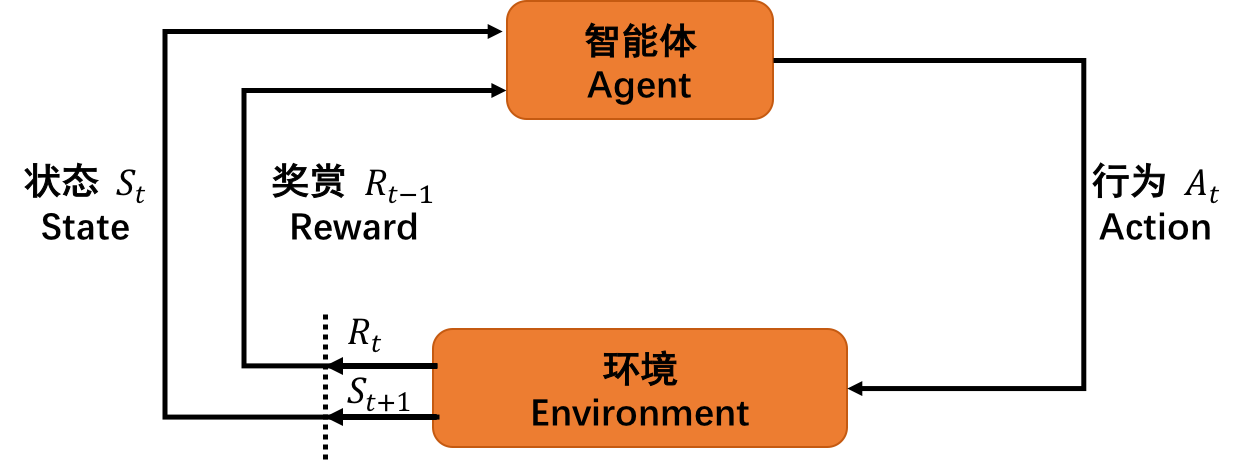
\includegraphics[width=0.8\textwidth]{强化学习过程_}
% \caption{强化学习的交互过程}
% \label{fig:强化学习过程_}
% \end{figure}

(a)首先,Agent要感知当前的环境状态(state);

(b)然后,根据当前的状态并结合上一刻获得的奖赏值(reward,强化信号),Agent会从行为集合中选择一个行为(action)并执行;

(c)接着,当Agent执行完行为后,环境会转移到下一个新状态并会反馈出新的奖赏信息;

(d)最后,Agent根据环境反馈的奖赏信息,计算出回报值(return),并将该回报值作为更新内部策略的依据。

 在这一过程中,Agent并不会被告知应该采取哪个行为,而只能经过不断的尝试后,根据得到的环境反馈信息做出判断。Agent选择行为的原则是:所选择的行为应该在以后的学习过程受到环境奖励的概率增大,受到惩罚(负奖赏)的概率减小,也就是说,当前采取的行为只与最终的目标有关。因为在序贯决策中,奖励信号是有延迟的,所以Agent有时候宁愿会牺牲即时(短期)的奖励以获取更多的长期奖励。从以上分析中可以看出,试错搜索(trial-and-error search)以及延迟回报(delay return)是强化学习最显著的特征\citep{张文旭2017基于事件驱动的多智能体强化学习研究}。

 与机器学习中的监督学习方法不同,一方面,强化学习在学习过程中并不需要多样化的标签数据,而只需要带有奖赏信号的交互数据。另一方面,监督学习是通过将模型预测的输出值与样本标签之间误差,反馈给模型以指导模型的学习,而在强化学习过程中,由环境产生的奖赏信息仅仅被看作是对行为策略好坏的一种评价,Agent在行为策略与评价中获取知识,不断地改进行为策略以适应环境,并不会指导Agent如何去产生正确的动作。

 另外,根据优化目标的不同,可以将强化学习的求解方法分为基于值函数的方法和基于策略搜索的方法两类。其中,基于值函数的强化学习方法首先迭代地计算近似最优值函数,然后再根据该值函数来改善行为策略;而在策略搜索的方法中,直接对策略进行迭代。特别地,本文只针对基于值函数的方法进行研究,因此本章也只介绍与基于值函数强化学习方法相关的理论知识。

\section{强化学习的组成要素}
因为强化学习的理论框架是MDP,所以本节首先对MDP进行介绍,接着对强化学习的基本组成要素:策略、回报和值函数等概念进行详细阐述,以便后续开展对强化学习方法的讨论。

% 介绍马尔科夫决策过程,策略、累计回报、值函数、贝尔曼方程、最优值函数
\paragraph{马尔科夫决策过程}
一般使用MDP来对强化学习问题进行形式化的描述,进一步地,如果状态空间和行为空间都是有限的,则使用有限马尔科夫决策过程(finite Markov Decision Process, finite MDP)来描述\citep{2016连续空间强化学习研究}。本文所涉及的MDP除特别说明外,均指的是finite MDP。通常可以使用一个四元组$<\mathcal{S},\mathcal{A},p,r>$来表示finite MDP,其中:$\mathcal{S}$表示有限的状态空间,定义为一个有穷集合$\{ S_1,S_2,\cdots ,S_N \}$,$N$为状态空间的大小;$\mathcal{A}$表示有限的行为空间,定义为一个有穷集合$\{ A_1,A_2,\cdots ,A_M \}$,$M$为行为空间的大小;$p$表示状态转移函数;$r$表示即时奖赏函数。

考虑在MDP中任意的离散时间点$t$时,环境的状态为$S_{t}$,此刻Agent若采取行为$A_{t}$,便会得到有限的即时奖赏$R_{t}$,并且环境状态也会相应的发生改变,转移到下一状态$S_{t+1}$。其中,下一时刻的状态$S_{t+1}$是根据状态转移函数$p$来确定的,有限奖赏$R_{t}$是根据奖赏函数$r$求得的。

另外,根据状态转移方式的不同,可以分成确定性状态转移和随机性状态转移两种。其中,在确定性状态转移中,所转移到的下一状态是确定性的,其奖赏函数只和当下的状态和所要采取的行为有关,可以看成是对即时奖赏的一种评价。在随机性状态转移中,所转移到的下一状态是不确定的,而是一个随机变量,并且奖赏函数除了和当前状态和所采取的行为有关之外,还依赖于下一个状态,因此可以看作是对长期效果的评价。

% 如式\eqref{seq:p}和\eqref{seq:rr}:
% \begin{equation}\label{seq:p}
% p(s^{'}|s,a)=\bm{\text{Pr}}\{S_{t+1}=s|S_{t}=s,A_{t}=a\}
% \end{equation}
% \begin{equation}\label{seq:rr}
% r(s,a,s^{'})=\mathbb{E}[R_{t}|S_{t}=s,A_{t}=a,S_{t+1}=s^{'}]
% \end{equation}

% 其中,公式\eqref{seq:p}表示在给定状态s时,执行行为a后,环境状态转移到s^{'}的概率。公式\eqref{seq:rr}表示当前状态s和行为a时,环境转移到下一状态s^{'}所产生的期望奖赏。




% 又因为马尔科夫决策过程的状态具有马尔科夫性,因此状态转移函数和奖赏函数都仅和当前状态和行为有关,与历史的状态序列和行为序列无关。即:$p(s^{'},r|s,a) = Pr\{S_{t}=s^{'}, R_t=r|S_{t-1}=s, A_{t-1}=a\}$且$\sum_{s^{'}\in S}p(s^{'}|s,a)=1$,$\forall s\in S,\forall a\in A$。
\paragraph{策略和回报}
% \subparagraph{策略}
% 强化学习的目标是从给定的马尔科夫决策过程中,寻找最优的策略。
所谓策略,是指从状态$s$到行为$a$的映射,通常用符号$\pi$表示。
% 指在某一状态下,所采取的动作或所采取动作的概率,。
同样,策略也有确定性策略和随机性策略,其中,确定性策略定义为:$\pi$: $\mathcal{S} \to \mathcal{A}$ ,其输出的是一个动作序列,而随机性策略定义为:$\pi$: $\mathcal{S} \times \mathcal{A} \in [0,1]$ ,其输出的是该状态下所采取动作的概率:$\pi(s,a)=p[A_{t}=a|S_{t}=s]$。

% \subparagraph{回报}
强化学习的任务是从与环境的持续交互中,学习一个策略$\pi$,使其产生的累积奖赏(cumulative reward)最大化,即回报最大化。
% 当给定一个策略$\pi$时,如何进行策略的评估呢?此时便用到了累积奖赏的概念。
假设在时刻$t$后接收到的奖赏序列为$\{R_{t}, R_{t+1}, R_{t+2},\cdots\}$,那么采用折扣累积奖赏的方式计算回报可以表示为式\eqref{seq:reward}:

\begin{equation}\label{seq:reward}
G_{t}=\sum_{k=0}^{\infty}\gamma^{k}R_{t+k}
\end{equation}

式\eqref{seq:reward}中,$G_{t}$为回报,$\gamma<1$,为一个常量,称为折扣因子。特别地,在系统与环境的交互过程中,如果任务可以自然地被分为带有终止时间片的片段,则该任务称为情节式(episodes)任务。如果任务无法分解成若干片段,整个任务需要不断的进行下去,则该任务称为连续式(continous)任务。

\paragraph{值函数}

% 在Agent的学习过程中,当给定策略$\pi$时,考虑如何评价某一状态的价值。
因为强化学习的目标是追求累积奖赏最大化,所以很自然的想法是可以利用上述回报的计算方式来衡量某一状态的价值。但是,由于在某一状态下的产生的状态序列可以会有很多种,所以回报$G_{t}$是个随机变量,并不是一个确定的值,无法作为目标函数进行优化。然而,其期望是个确定值,因此可以作为状态值函数的定义:当Agent采取策略$\pi$时,其回报服从一个分布,将状态$s$的期望回报值定义为状态$s$的值函数。公式定义为\eqref{seq2_vs}:
\begin{equation}
\label{seq2_vs}
v_{\pi}(s)=\mathbb{E}_{\pi}[G_{t}|S_t=s]=\mathbb{E}_{\pi}[\sum_{k=0}^{\infty}\gamma^{k}R_{t+k}|S_t=s]
\end{equation}

% Q函数是另一种评估值函数的方法。Watkins指出:。

在某些情况下,记录状态行为的值比只记录状态的值更有用。所以,将在状态$s$下,Agent采取行为$a$后所产生回报的期望值定义为状态行为值函数,公式定义为\eqref{seq2_qsa}:
\begin{equation}
\label{seq2_qsa}
q_{\pi}(s,a)=\mathbb{E}_{\pi}[G_{t}|S_t=s,A_t=a]
=\mathbb{E}_{\pi}[\sum_{k=0}^{\infty}\gamma^{k}R_{t+k}|S_t=s,A_t=a]
\end{equation}

上述状态值函数\eqref{seq2_vs}的表达形式在实际计算和编程的时候很不方便,因此,可以经过进一步的推导,得到状态值函数的贝尔曼方程,如式\eqref{seq1}:
\begin{equation}
\label{seq1}
\begin{aligned}
v_{\pi}(s)&=\mathbb{E}_{\pi}[G_{t}|S_t=s]\\
&=\mathbb{E}_{\pi}[\sum_{k=0}^{\infty}\gamma^{k}R_{t+k} | S_t=s]\\
&=\mathbb{E}_{\pi}[R_{t} + \gamma \sum_{k=0}^{\infty}\gamma^{k}R_{t+k+1}|S_t=s]\\
&=\sum_{a}\pi(a|s)\sum_{s^{'}}p(s^{'}|s,a)[r(s,a,s^{'}) + \gamma \mathbb{E}_{\pi}[\sum_{k=0}^{\infty}\gamma^{k} R_{t+k+1} |S_{t+1}=s^{'}]]\\
&=\sum_{a}\pi(a|s)\sum_{s^{'}}p(s^{'}|s,a)[r(s,a,s^{'})+\gamma v_{\pi}(s^{'})], \forall s \in S
\end{aligned}
\end{equation}

在式\eqref{seq1}中,$p(s^{'}|s,a) = \bm{\text{Pr}}\{S_{t+1}=s^{'}|S_{t}=s, A_{t}=a\}$,表示在状态$s$下Agent执行行为$a$后,环境转移到下一个状态$s^{'}$的概率。$r(s,a,s^{'})=\mathbb{E}[R_{t}|S_{t}=s,A_{t}=a,S_{t+1}=s^{'}]
$,表示在给定当前状态$s$下,当Agent采取行为$a$后,环境转移到下一状态$s^{'}$时所产生的期望奖赏。

同样的方法也可以得到状态行为值函数的贝尔曼方程,如公式\eqref{seq2}所示:
\begin{equation}
\label{seq2}
\begin{aligned}
q_{\pi}(s,a)=\sum_{s^{'}}p(s^{'}|s,a)[r(s,a,s^{'})+ \gamma \sum_{a'}\pi(a^{'}|s^{'}) q_{\pi}(s^{'},a^{'})], \forall s \in S, \forall a \in A
\end{aligned}
\end{equation}

计算值函数的目的是为了构建学习算法时从数据中学习到最优的策略。因为每个策略都对应着一个状态值函数,那么最优策略就对应着最优的状态值函数。因此,将最优状态值函数$v_{*}(s)$定义为所有策略中值最大的那个值函数,即$v_{*}(s)==\max_{\pi}v_{\pi}(s)$,同样地,将最优状态行为值函数$q_{*}(s,a)$定义为所有策略中值最大的那个状态行为值函数,即$q_{*}(s,a)=\max_{\pi}q_{\pi}(s,a)$

因此,将公式\eqref{seq1}和公式\eqref{seq2}进行推导,又可以分别得到最优状态值函数$v_{*}(s)$和最优状态行为值函数$q_{*}(s,a)$的贝尔曼最优方程如式\eqref{seq21}和\eqref{seq22}所示(因为篇幅限制,推导过程略):
\begin{equation}\label{seq21}
\begin{aligned}
v_{*}(s)=\max_{a}\sum_{s^{'}}p(s^{'}|s,a)[r(s,a,s^{'})+\gamma v_{*}(s^{'})]
\end{aligned}
\end{equation}
\begin{equation}\label{seq22}
\begin{aligned}
q_{*}(s,a)=\sum_{s^{'}}p(s^{'}|s,a)[r(s,a,s^{'}) +\gamma \max_{a'} q_{*}(s^{'},a^{'})]
\end{aligned}
\end{equation}

最后,若求出了最优状态行为值函数,最优策略可以通过直接最大化 $q_{*}(s,a)$来决定,如式\eqref{seq23}:
\begin{equation}\label{seq23}
\begin{aligned}
\pi_{*}(a|s) = 
    \begin{cases}
        1 & if \ a=\argmax_{a\in A}{q^{*}(s,a)},\\
        0 & otherwise.
    \end{cases}
\end{aligned}
\end{equation}

最后,需要强调的是:从公式\eqref{seq2_vs}和公式\eqref{seq2_qsa}可以看出,值函数其实是对未来奖赏(回报)的一种预测。那么,对于一个状态$s$,如果它此时所获得的即时奖赏比较低,并不代表它的状态值就低,因为假如在状态$s$之后的状态里产生了更高的奖赏,那么它依旧会取得很高的状态值,这就是强化学习在学习过程中可以考虑长期收益最大化的原因,也是本文选择使用强化学习技术应用于营销问题以获取长期收益最大化的原因。

% 但是,因为值函数的计算需要考虑到其后续状态的情况,所以
% 求解值函数需要Agent在其整个生命周期内通过一系列的观察和不断的估计才能得到。
所以,接下来的工作就是如何快速而准确地进行最优值函数的求解,进而求得最优的策略。

\section{基于值函数的强化学习算法}

根据强化学习在求解过程中是否需要环境,可以分为基于模型(model-based)的动态规划法和模型无关(model-free)的强化学习方法。其中,在基于模型的动态规划法中,需要提供精确的环境模型,然后根据环境的动态性利用贝尔曼方程迭代的求解值函数。模型无关的强化学习算法则不需要提供环境模型,而是直接利用收集到的数据求解状态值函数和状态行为值函数。模型无关的强化学习算法包括蒙特卡罗(Monte Carlo, MC)法和时间差分(Temporal Difference, TD)法\citep{2016面向强化学习的模型学习算法研究}。

\subsection{动态规划法}
动态规划法是在给定环境模型的情况下,求解值函数和最优策略的方法,在实际应用虽然有很大的局限性,但它是研究强化学习方法的理论基础。根据迭代方式的不同,动态规划法又可分为策略迭代(Policy Iteration)和值迭代( Value Iteration)两种方法。
\paragraph{策略迭代}

策略迭代法主要包括策略评估和策略改善两步,并且这两步在学习的过程中依次交替进行。具体地,当进行策略评估的时候,算法每轮都需要进行多次迭代,并且在每次迭代时,需要根据上一轮改善后的策略对状态空间里的每个状态进行扫描,然后使用贝尔曼方程进行状态值的更新,经过不断地迭代后,使值函数最终收敛至不动点,进入这一轮的策略改善步骤。在进行策略改善的时候,算法利用上一轮策略评估得到的值函数,以贪心的方式生成一个新的策略。接着,不断循环以上两个步骤,直至策略收敛至最优策略。特别地,在进行策略评估的时候,公式$\eqref{seq1}$中状态值$v_{\pi}(s)$的计算需要利用其后继状态的值函数$v_{\pi}(s^{'})$,所以,用到了自举(Bootstrapping)的思想。

下面,以状态行为值函数的策略迭代过程为例,进行详细的介绍:
\begin{displaymath}
\begin{aligned}
\pi_{0}\xrightarrow{E}q_{\pi_0}\xrightarrow{I}\pi_{1}\xrightarrow{E}q_{\pi_1}\xrightarrow{I}\pi_{2}\xrightarrow{E}q_{\pi_2}\xrightarrow{I}\pi_{3}\xrightarrow{E} \cdots \xrightarrow{I}\pi_{*}\xrightarrow{E}q_{\pi_{*}}
\end{aligned}
\end{displaymath}

其中,$E$代表策略评估过程,$I$代表策略改善过程。初始时,策略和值函数都是随机的。在策略评估时,针对每一个状态行为值,使用贝尔曼方程进行值函数的更新,直到$q_{k+1}$稳定便结束本轮迭代,如式\eqref{seq:beierman2}所示,其中$k$表示本轮迭代的次数。
\begin{equation}\label{seq:beierman2}
\begin{aligned}
q_{k+1}(s,a)=\sum_{s^{'}}p(s^{'}|s,a)[r(s,a,s^{'})+ \gamma \sum_{a'}\pi(a^{'}|s^{'}) q_{k}(s^{'},a^{'})]
% q_{k+1}(s,a)=\sum_{s^{'},r}p(s^{'},r|s,a)[r+\gamma \sum_{a'}\pi(a^{'}|s^{'}) q_{k}(s^{'},a^{'})]
\end{aligned}
\end{equation}

在策略改善时,对每一个状态,使用贪婪策略对当前策略进行改善,如\eqref{seq:beierman3}所示。
\begin{equation}\label{seq:beierman3}
\begin{aligned}
\pi(s)=\argmax_{a}q(s,a)
\end{aligned}
\end{equation}

在收敛到最优策略之前,每一轮的策略都好于前一轮的策略。当策略$\pi$稳定时,动态规划过程结束,即可得到最优值函数$q_{*}(s,a)$和最优策略$\pi_{*}$。
\paragraph{值迭代}

值迭代算法是对策略迭代算法过程的简化,同样也包括策略评估和策略改善两个步骤。与策略迭代不同的是,在进行策略改善的时候,它不需要等到值函数完全收敛时才进行改善,而是对全部的状态行为空间每进行一次扫描(更新)就进行一次策略改善,通过这种方式,加快了值函数的收敛速度。对每一个状态行为对,值迭代的更新公式如式\eqref{seq:beierman4},其中$l$为迭代的轮数。:
\begin{equation}
\begin{aligned}\label{seq:beierman4}
q_{l+1}(s,a)=\sum_{s^{'}}p(s^{'}|s,a)[r(s,a,s^{'})+ \gamma \max_{a^{'}} q_{l}(s^{'},a^{'})]
% q_{k+1}(s,a)=\sum_{s^{'},r}p(s^{'},r|s,a)[r+\gamma \max_{a^{'}} q_{k}(s^{'},a^{'})]
\end{aligned}
\end{equation}

直到$q_{l+1}$稳定,算法结束。此时因为值函数已经收敛,直接对值函数使用贪心方法就可以得到最优策略。

\subsection{蒙特卡洛方法}
由公式\eqref{seq:beierman2}和公式\eqref{seq:beierman3}可以看出,动态规划法在求解值函数时需要提供完整的环境模型(状态转移概率)且计算代价太大,限制了其在实际场景中的应用。于是就出现了模型无关的算法:蒙特卡罗方法。

蒙特卡罗方法采用了经验平均的思想来代替随机变量的思想,因而不再需要提供环境模型。其中,经验是指按照该策略做了很多次实验,产生很多情节(episode),每一个情节就是一次实验,平均就是指的平均值,按照求解方法不同又可以分为第一次访问(first-visit)蒙特卡罗方法和每次访问(every-visit)蒙特卡罗方法。在与环境的交互过程中,当一个情节结束后,MC便会用情节中的数据进行值函数的更新和策略的改善。另外,值函数的更新使用可递增(Incremental )计算均值的方法,以状态值函数为例,更新公式为\eqref{seq:mc}:
\begin{equation}\label{seq:mc}
\begin{aligned}
V_{k+1}(S_{t})=V_{k}(S_{t})+ \alpha(G_{t}-V_{k}(S_{t}))
\end{aligned}
\end{equation}

其中,$V_{k+1}(S_{t})$表示第$k+1$次迭代时$v_{k+1}(S_{t})$估计值,$\alpha$表示学习率,$G_{t}$表示从状态$s$开始到情节结束所获的的期望奖赏。

在动态规划中,为了保证值函数的收敛,算法会扫描状态空间的每一个状态。而蒙特卡罗方法想要充分评估值函数的前提是保证每个状态都可以被访问到,因此MC采用了探索性初始化(Exploring Start, ES)的方法,即在每一个情节在迭代时,其初始状态都是随机分配的。

\subsection{时间差分方法}
相比于动态规划法,蒙特卡罗法使用了经验平均的思想,虽然摆脱了对模型的依赖,但是必须要等到每个情节结束后才可以进行值函数评估和策略更新,所以学习速度慢,学习效率不高。而动态规划因为使用了bootstrapping思想,可以在情节未结束时就可以根据未来值函数估计当前的值函数。时间差分法综合了两者的优点,融合了蒙特卡罗的采样方法和动态规划的bootstrapping思想。

所谓时间差分是指对同一事件或变量在连续两个时刻观测的偏差。在本文中,除特别说明外,所提到的时间差分算法均是指的一步更新算法,即值函数直接根据下一个时间步进行学习,进而估计下一个状态的值函数。假设在状态$S_{t}$时,Agent采取行为$A_{t}$,获得奖赏$R_{t}$的同时状态转移到$S_{t+1}$。
% 因为环境从状态$S_{t}$向$S_{t+1}$以外的其它状态转移的概率为0,设$V(S_{t})$为最优$v_{*}(S_{t})$的估计值,那么状态$S_{t}$的值函数为:
% \begin{equation}
% \begin{aligned}
% V(S_{t})=R_{t+1}+\gamma V(S_{t+1})
% \end{aligned}
% \end{equation}
那么,时刻$t$的时间差分$\delta_{t}$可表示为\eqref{shijiachafen}:
\begin{equation}\label{shijiachafen}
\begin{aligned}
\delta_{t}=R_{t}+\gamma V(S_{t+1})-V(S_{t})
\end{aligned}
\end{equation}

值函数的更新公式可表示为\eqref{shijiachafen2}:
\begin{equation}\label{shijiachafen2}
\begin{aligned}
V(S_{t}) \gets V(S_{t})+\alpha (R_{t}+\gamma V(S_{t+1})-V(S_{t}))
\end{aligned}
\end{equation}

在式\eqref{shijiachafen2}中,$\alpha$为步长参数,控制学习率。$R_{t}+\gamma V(S_{t+1})$称为TD目标,与式\eqref{seq:mc}中的$G_{t}$相对应,两者不同之处在于TD目标利用了bootstrapping方法估计当前值函数。

另外,根据探索策略(行为策略)和评估策略是否为一个策略,可以将强化学习方法分为同策略(on-policy)和异策略(off-policy)两种方法。同样,时间差分方法也包括了同策略的Sarsa方法和异策略的Q-learning方法。在Sarsa方法中,行动策略和评估策略都是$\epsilon-greedy$的方法,对应的算法伪代码如$\ref{algo:algorithm_1}$所示。其中$\epsilon-greedy$方法是指,当给定一个$0$到$1$之间的数$\epsilon$后,以$\epsilon$的概率随机选择行为,以$1-\epsilon$的概率选择最好的行为:$\pi(S_{t})=\argmax_{a} Q(S_{t},a)$。

\begin{algorithm}[htbp]
\small
\SetAlgoLined
\SetKwRepeat{Repeat}{Repeat}{until} 
% \KwData{this text}
% \KwResult{how to write algorithm with \LaTeX2e }
初始化$Q(s,a)$,$\forall s \in \mathcal{S}$,$\forall a \in \mathcal{A}$, 给定参数$\alpha$,$\gamma$\;
\Repeat{所有的$Q(s,a)$收敛}{
初始化起始状态$s$\;
根据$\epsilon-greedy$策略在状态$s$下选择行为$a$\;
\Repeat((对每个情节的每一步)){$s$是终止状态}{
	在状态$s$下选择行为$a$,得到奖赏$r$和下一个状态$s^{'}$\;
	在状态$s^{'}$下根据$\epsilon-greedy$策略选择动作$a^{'}$\;
	$Q(s,a) \gets Q(s,a)+\alpha[r+\gamma Q(s^{'},a^{'}) - Q(s,a)]$\;
	$s=s^{'}$,$a=a^{'}$\;
	}
}
输出最终策略:$\pi(s)=\argmax_{a}Q(s,a)$\;
\caption{Sarsa算法}
\label{algo:algorithm_1}
\end{algorithm}

与Sarsa方法不同,在Q-learning方法中,行为策略采用$\epsilon-greedy$策略,而目标策略采用贪婪策略,故又称为异策略Q-learning算法,其伪代码如$\ref{algo:algorithm_2}$所示。
\begin{algorithm}[htbp]
\small
\SetAlgoLined
\SetKwRepeat{Repeat}{repeat}{until} 
% \SetAlgoRefName{algorithm_2}
初始化$Q(s,a)$,$\forall s \in \mathcal{S}$,$\forall a \in \mathcal{A}$, 给定参数$\alpha$,$\gamma$\;
\Repeat{所有的$Q(s,a)$收敛}{
初始化起始状态$s$\;
% 根据$\epsilon-greedy$策略在状态$s$下选择行为$a$\;
\Repeat((对每个情节的每一步)){$s$是终止状态}{
	在Q函数中,根据$\epsilon-greedy$策略在状态$s$下选择行为$a$\;
	执行行为$a$后,得到回报$r$和下一状态$s^{'}$\;
	$Q(s,a) \gets Q(s,a)+\alpha[r+\gamma \max_{a} Q(s^{'},a)-Q(s,a)]$\;
	$s=s^{'}$\;
	}
}
输出最终策略:$\pi(s)=\argmax_{a}Q(s,a)$\;
\caption{Q-learning算法}
\label{algo:algorithm_2}
\end{algorithm}

% 在TD(0)中,更新当前值函数时,只用到了下一步状态值函数。而TD($\lambda$)考虑从未来的多步进行学习,并且采用加权的方法融合这多步的估计值,$\lambda \in [0,1]$决定了向未来观察的时间步长度。即
% \begin{equation}
% \begin{aligned}
% V(S_{t} )\gets V(S_{t})+\alpha (G^{(\lambda)}_{t}-V(S_{t}))
% \end{aligned}
% \end{equation}
% 其中,
% \begin{displaymath}
% \begin{aligned}
% G^{(\lambda)}_{t}=(1-\lambda) \sum_{n=1}^{\infty} \lambda^{n-1} G^{(n)}_{t}\\
% \end{aligned}
% \end{displaymath}
% \begin{displaymath}
% \begin{aligned}
% G^{(n)}_{t}=R_{t+1}+\gamma R_{t+1}+ \cdots +\gamma^{n-1} R_{t+n}+\gamma^{n} V(S_{t+n})
% \end{aligned}
% \end{displaymath}

% 这就是TD($\lambda$)的前向视角表达形式,但是,这种方式需要等到整个实验结束才能计算。后向视角利用增量式的更新方式,不需要等到实验结束就可以更新当前状态的值函数,并且引入了资格迹$Z_{t}(s)$的概念,资格迹记录了最近被访问过的状态,也就是说,最近且最频繁被访问到的状态会被赋予最大的“资格”。更新方式为:

% (1)首先,计算当前状态的TD偏差:$\delta_{t}=R_{t+1}+\gamma V(S_{t+1})-V(S_{t})$

% (2)其次,更新资格迹:$Z_{t}(s) = 
%     \begin{cases}
%         \gamma \lambda Z_{t-1} & if s \neq s_{t},\\
%         \gamma \lambda Z_{t-1}+1 & if s = s_{t}.
%     \end{cases}$

% (3)最后,对状态空间中的每个状态$s$,更新值函数:$V(s) \gets V(s)+\alpha \delta_{t} Z_{t}(s)$

% 综上,后向视角的时间差分方法不仅不需要环境模型,而且利用了增量在线的机制,实现方式简单有效,同时也保证了策略的实时性,被认为是强化学习中最核心的算法。

\section{值函数的逼近方法}
至此,可以归纳出求解基于值函数的强化学习算法的基本步骤是:首先进行近似最优值函数的评估,然后再利用该值函数改善当前的策略。其中,值函数的评估是关键。

在之前所介绍的强化学习方法中,值函数其实是一个表格,其索引是状态或者状态行为对,值迭代更新实际上就是这张表格的迭代更新,因此,这种强化学习称为表格型强化学习,它有一个前提条件:状态空间和行为空间都是离散的且空间大小不能太大。然而,现实中的很多问题都具有很大的状态(行为)空间,甚至是连续的状态(行为)空间,比如围棋有 $10^{170}$  个状态空间,控制直升机飞行需要的是一个连续的状态空间。在这种情况下,可以使用函数逼近的方法表示值函数。

从数学的角度来看,函数逼近方法有参数化函数逼近方法和非参数化函数逼近方法,其中参数化函数逼近又可以分成线性函数逼近和非线性函数逼近两种\citep{强化学习中值函数逼近方法的研究}。

\subsection{参数化函数逼近}

\paragraph{参数化线性函数逼近}
参数化函数逼近可以定义为从参数空间到近似值函数空间的一种映射\citep{强化学习中值函数逼近方法的研究}。因此,状态和状态行为值函数可以分别由一组参数$\bm{\theta}\in \mathbb{R}^{n} $ 来近似表示,在本文中,将近似状态值函数和近似状态行为值函数分别记为:$\hat{v}(s;\bm{\theta})$和$\hat{q}(s,a;\bm{\theta})$,如\eqref{seq_2_3_2}所示。
% 函数的形式和参数的个数事先由先验知识预设,而且参数是通过与目标函数有关样本数据来调整的。
\begin{equation}
\label{seq_2_3_2}
\begin{aligned}
&\hat{v}(s;\bm{\theta})\approx v_{\pi}(s)\\
&\hat{q}(s,a;\bm{\theta})\approx q_{\pi}(s,a)
\end{aligned}
\end{equation}

从上式$\eqref{seq_2_3_2}$中,可以发现,在近似的状态值函数$\hat{v}(s;\bm{\theta})$中,针对每个状态,不再存储其状态值,而是只存储一组参数。把从已知的状态中得到的值函数,推广至那些未碰及的状态中,这对于拥有大规模的状态空间来说,相当于对其状态空间进行了压缩。由于 $\bm{\theta}\in \mathbb{R}^{n}$,因此空间存储开销为$O(n)$,当状态规模较大且均为离散时,$n$远远小于为每个状态存储值的开销$|\mathcal{S}|$。

当近似的函数结构
% ($\hat{v}(s;\bm{\theta})$和$\hat{q}(s,a;\bm{\theta})$)
确定后,对值函数的更新就相当于对参数的更新。那么,此时就需要利用实验数据来更新参数值。但是,强化学习中没有标签数据,如何才能从数据中学到值函数呢?

从基于表格的值函数更新过程中可以看出,无论是MC方法还是TD方法,都是朝着某一个目标值更新的,这个目标值在蒙特卡罗方法中是$G_{t}$,在时间差分方法中是$R_{t}+\gamma Q(S_{t+1},A_{t+1})$
% ,在$TD(\lambda)$中是$G^{\lambda}_{t}$
。所以,如果将表格型值函数的更新过程推广至值函数逼近过程,那么,逼近值函数$\hat{v}(s;\bm{\theta})$的过程实际上可以看作是一个监督学习的过程,其数据和标签对为$<S_{t}, v_{\pi}(S_{t})>$,其中$v_{\pi}(S_{t})$等价于蒙特卡罗方法中的$G_{t}$,时间差分方法中的$R_{t}+\gamma Q(S_{t+1},A_{t+1})$
% ,以及$TD(\lambda)$中是$G^{\lambda}_{t}$
。
% 因此,只要将公式$\eqref{seq:gradient}$总的$v_{\pi}(S_{t})$做相应替换就可以进行求解了。
那么,以状态值函数的逼近为例,需要训练的目标函数可表示为\eqref{seq:fun_approxi_obj}的形式:
\begin{equation}
\label{seq:fun_approxi_obj}
\begin{aligned}
\argmin_{\bm{\theta}}(v_{\pi}(s)-\hat{v}(s;\bm{\theta}))^2
\end{aligned}
\end{equation}

即通过寻找参数向量$\bm{\theta}$,最小化近似值函数$\hat{v}(s;\bm{\theta})$与真实值函数$v_{\pi}(s)$的均方差。另外,根据更新方式的不同,值函数的更新方法可以分为增量式更新方法和批更新方法。

在增量式更新方法中最常用的是随机梯度下降法,所以,由公式$\eqref{seq:fun_approxi_obj}$,利用随机梯度下降法,可以得到参数的更新公式为\eqref{deq:suijitidu}:
\begin{equation}\label{deq:suijitidu}
\begin{aligned}
\bm{\theta}_{t+1} \gets \bm{\theta}_{t} + \alpha[v_{\pi}(s)-\hat{v}(S_{t};\bm{\theta})]\triangledown_{\theta} \hat{v}(S_{t};\bm{\theta})
\end{aligned}
\end{equation}

% 进而,得到值函数参数的更新如下:
% \begin{equation}
% \label{seq:gradient}
% \begin{aligned}
% \triangle \bm{\theta} = \alpha [v_{\pi}(s)-\hat{v}(s;\bm{\theta})] \triangledown_{\theta} \hat{v}(s;\bm
% {\theta})
% \end{aligned}
% \end{equation}

% 然而,公式$\eqref{seq:gradient}$并不能直接用于强化学习中,因为公式里有一个真实价值函数$v_{\pi}(s)$,或者是一个具体的数值,而强化学习没有监督数据。

在增量式的学习方法中,每次更新模型需要与环境交互,数据使用一次即抛弃,导致样本使用效率不高。而所谓批更新方法是从给定一段时期的经验中抽取数据集:$D=\{<S_{1},v^{\pi}_{1}>,<S_{2},v^{\pi}_{2}>,\cdots,<S_{T},v^{\pi}_{T}>\}$,找到最好的拟合函数$\hat{v}(s;\bm{\theta})$,使的$LS(\bm{\theta})=\sum_{t=1}^{T}(v^{\pi}_{t}-\hat{v}^{\pi}_{t}(S_{t},\bm{\theta}))^2$ 最小,这种方法相当于经历重现(Experience Replay),把一段时期内的经历重新过一遍,更新参数,因此样本的利用效率高。

% 参数化函数逼近根据所使用逼近函数的不同,可分为参数化线性函数逼近和参数化非线性函数逼近两种。
以状态值函数为例,线性函数逼近方法可以表示为:
\begin{equation}
\begin{aligned}
\hat{v}(s;\bm{\theta})=\sum^{n}_{i=1}\phi_{i}(s) \bm{\theta}_{i}=\bm{\theta }^{T} \bm{\phi}(s)
\end{aligned}
\end{equation}

其中,$\bm{\theta}=(\bm{\theta}_{1},\cdots,\bm{\theta}_{n}) \in \mathbb{R}$,$\bm{\phi}(s)=(\phi_{1}(s),\cdots,\phi_{n}(s))^{T}$为状态$s$的特征向量,$\phi_{i}(s)$称为特征函数或者称为基函数,常见的基函数有:多项式基函数、傅立叶基函数以及径向基函数等。线性函数逼近方法不但原理简单易懂而且可以理论收敛到全局最优,缺点是表征能力较弱,而且基函数的种类和参数个数需要事先指定,限制了函数的逼近能力。
% 但是正是由于其具备良好的收敛性和理论简单性,在强化学习的参数化方法中得到了充分应用。


\paragraph{参数化非线性函数逼近}
在非线性函数逼近方法中,逼近函数是关于参数$\bm{\theta}$的非线性函数。在众多的非线性方法中,因为神经网络关于状态是可导的而且可以迭代求解,所以是强化学习中最适合的非线性函数逼近器。

神经网络可以也看作一种参数化基函数的方法,由于基函数的参数是从数据中学习得到的,因此其表示能力大大提升,神经网络的每层都可看成是基于上一层的新的基函数,也就是特征。从这个意义上说,后面一层是前一层的抽象,从而可以对高维输入达到降维的效果。所以,和线性逼近器相比,神经网络的优点是有很强的表征能力和逼近能力,可以对目标函数以任意精度逼近,但是也面临着许多问题:深度学习的样本之间是独立的,且目标分布是固定的,而强化学习前后的状态是相关的,并且目标分布在一直变化,往往会出现收敛不稳定等问题。因此,需要一个适用于非静态、非独立均匀分布的数据的训练方法来得到近似函数。

针对以上问题,基于Q-learning算法DeepMind团队提出了解决方法。1)使用卷积神经网络(Convolutional Neural Network, CNN)进行值函数的逼近;2)通过经验回放机制来解决强化学习中相关性以及非静态分布的问题;3)通过设置独立目标网络(TargetNet)来单独处理时间差分算法中的TD偏差,进一步降低数据之间的关联性,从而削弱收敛不稳定的问题。这就是DQN模型的主要内容,因为本文第四章的模型主要基于DQN模型的,所以,此处将这三个改进点进行介绍。

% 在强化学习的应用场景中,状态数据是可能是持续流入的,而且下一个状态通常与前一个状态是高度相关的。
% 但是其收敛性难以保证,容易陷入局部最优,使的学术界对其的研究停滞了很长时间,直到2013年,DeepMind团队提出了一些改进的深度强化学习的训练方法,很大程度上解决了神经网络在强化学习问题中的收敛性问题,并且取得了令人振奋的实验表现,引发了针对此问题的新的研究热潮。具体细节可以参见本文第三章关于DQN的介绍。深度神经网络就是其中一种参数化非线性函数逼近器,它不但可以高效的解决高维且连续的问题,而且还可以从数据中自动提取复杂的特征,于是出现了很多基于深度学习的深度强化学习(Deep Reinforcement Learning, DRL)技术。深度神经网络和强化学习技术的完美结合,可以利用神经网络强大的非线性逼近能力,让强化学习更好的进行Q值函数的学习,这种结合虽然可以在一定程度上达到优势互补的作用,但是也面临着许多问题。1)深度学习需要大量带标签的样本进行训练,而强化学习只有奖赏的返回值,并且存在奖赏延迟
% 在众多DRL模型中,以DQN模型最具代表性,因为它解决了DRL中一些一直以来悬而未解的关键问题,才使得深度强化学习以惊艳的表现重新回到大众的视野中。

 \subparagraph{卷积神经网络逼近值函数与构造标签}
图\ref{fig:CNN_DQN}为DQN模型逼近Q值函数时所使用的深度卷积神经网络的结构,它包含两个卷积层加两个全连接层。利用神经网络逼近值函数,不仅具有很强的表征能力,而且还可以自动地提取复杂特征。此处的Q值函数对应着一组参数,也就是神经网络中每层网络的权重,可以用向量$\bm{\theta}$表示,对应的值函数可以表示为$Q(s,a;\bm{\theta})$,所以对值函数的更新也就是对参数向量$\bm{\theta}$的更新。
\begin{figure}[htbp]
\centering
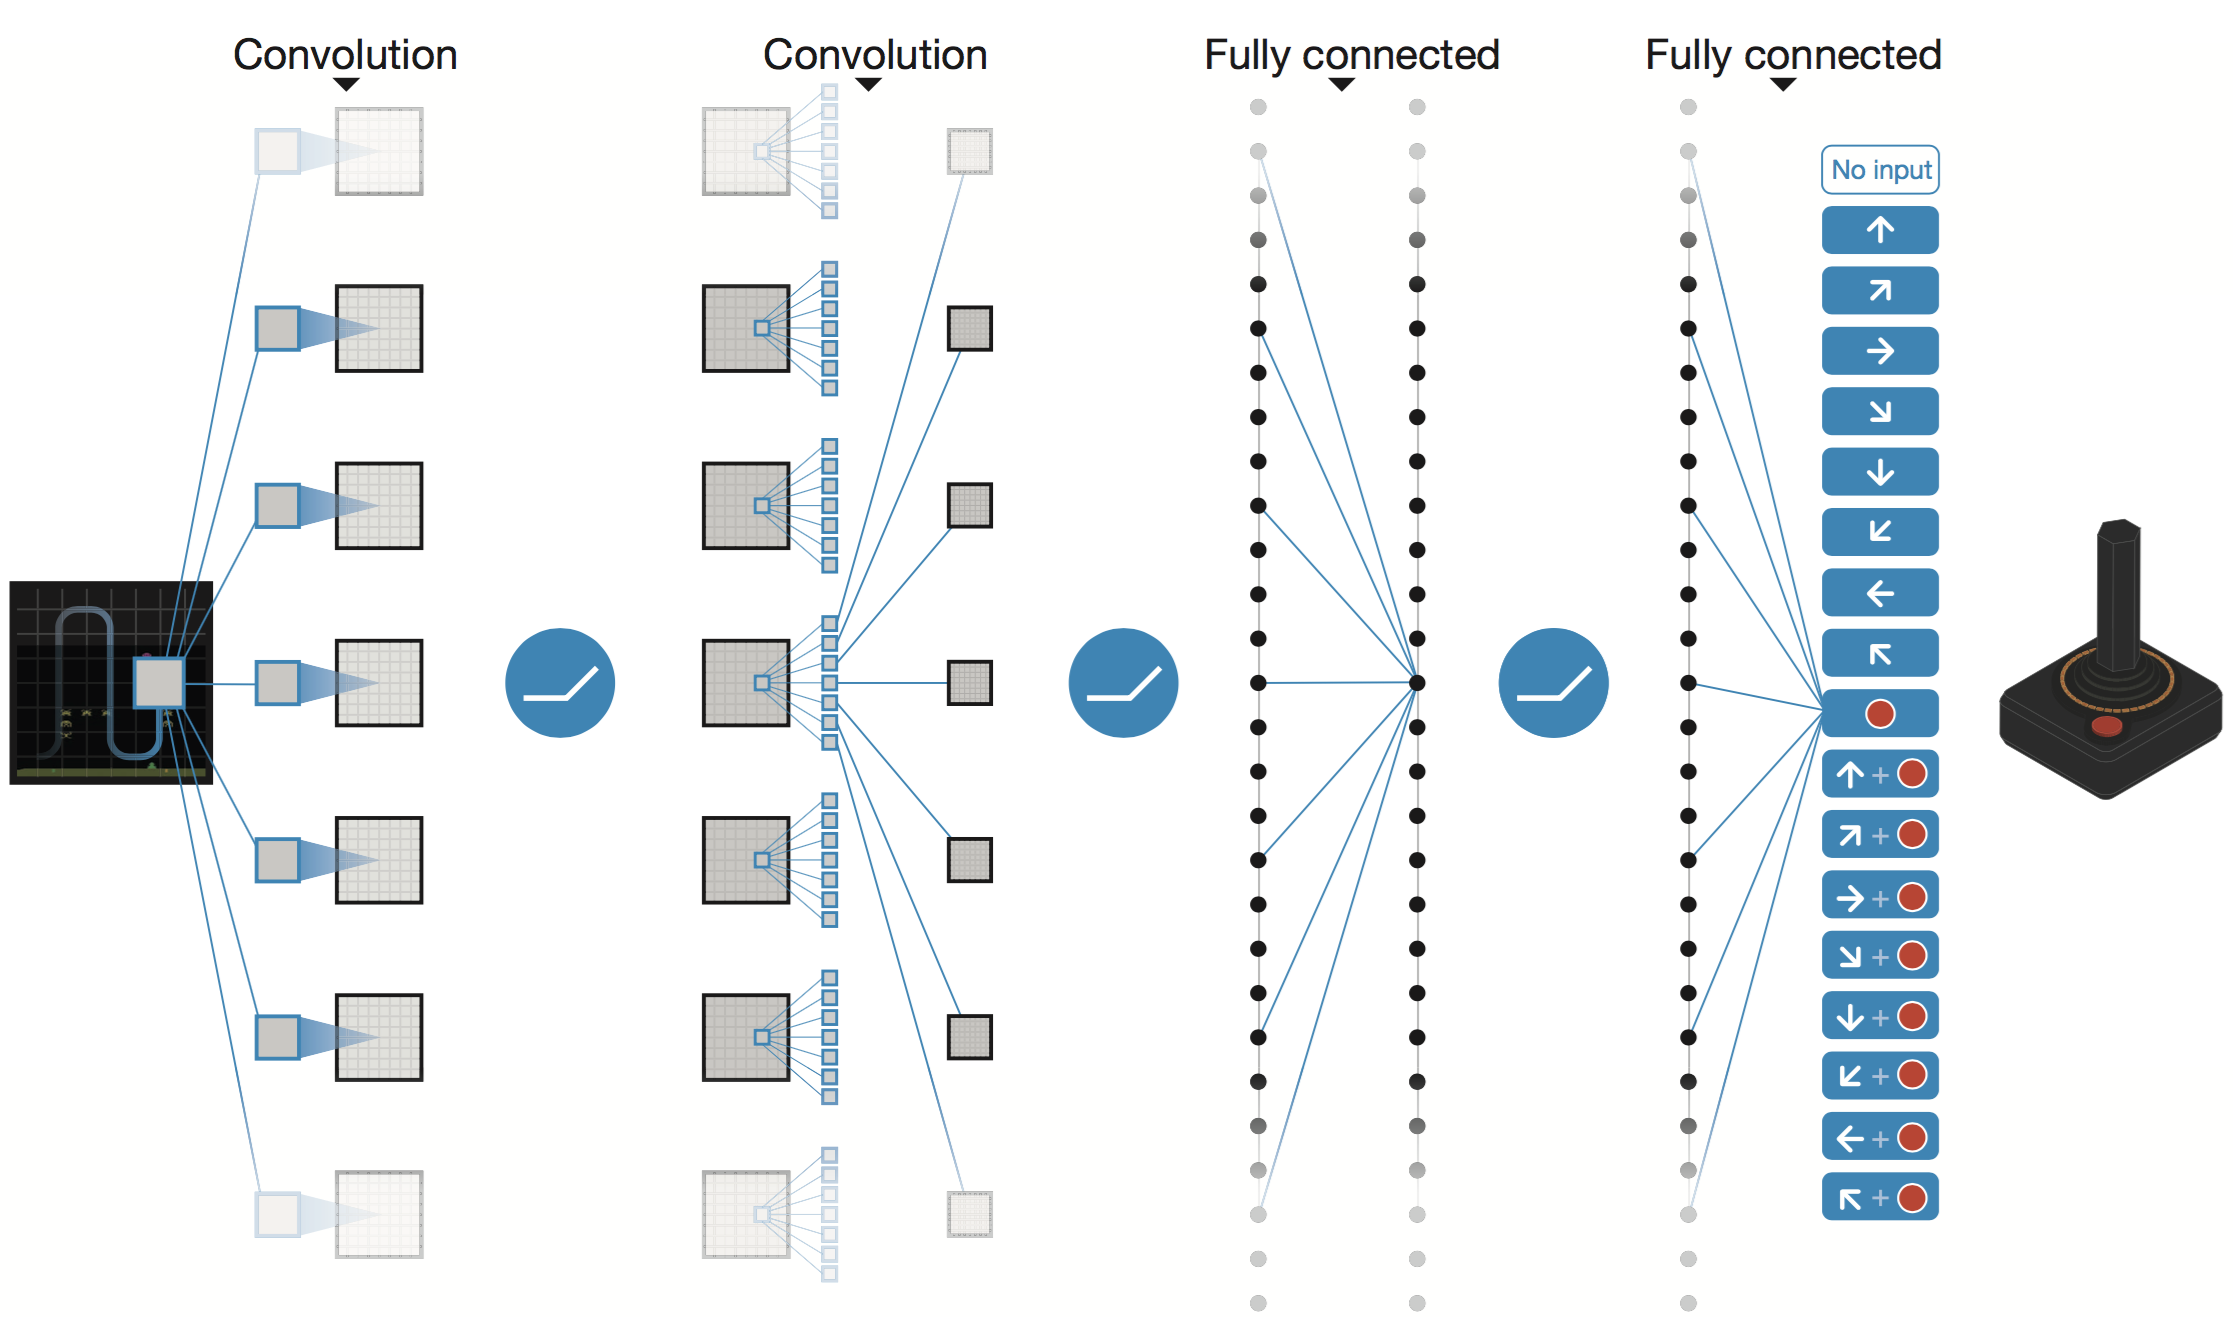
\includegraphics[width=1.0\textwidth]{CNN_DQN}
\caption{DQN模型中值函数的网络结构}
\label{fig:CNN_DQN}
\end{figure}

神经网络的训练是一个最优化过程,目的是让损失函数最小化,而损失函数是标签和网络输出的偏差。为此,需要巨量的带有标签的数据,然后通过反向传播使用梯度下降的方法来更新神经网络的参数。然而,Q-learning算法只有奖赏的返回值,参考上文的描述,可以使用Q目标值作为标签进行训练。

在算法$\ref{algo:algorithm_2}$中,Q的目标值是$r+\gamma \max_{a}Q(s^{'},a)$,而Q值函数学习的目的就是趋近该目标值。因此,DQN网络的损失函数可表示为:
\begin{equation}
\label{seq_3_2_1}
\begin{aligned}
L(\theta)=\mathbb{E}[(\underbrace{r+\gamma\max_{a^{'}} Q(s^{'},a^{'};\bm{\theta})}_{Target}-Q(s,a;\bm{\theta}))^{2}]
\end{aligned}
\end{equation}

在公式$\eqref{seq_3_2_1}$中,$s^{'}$,$a^{'}$分别表示下一个状态和下一个时刻将要采取的行为。
% 这里使用Q-learning要更新的Q值值函数作为目标值。有了目标值,又有当前值,那么偏差就能通过均方差来进行计算了。
接着,就可以按照参数化函数逼近的训练步骤,先求出损失函数的梯度,然后利用随机梯度下降法(Stochastic Gradient Descent, SGD)来更新参数,从而得到最优的Q值函数了。

其实,早在1995年Bertsekas等人就将神经网络应用在强化学习的值函数逼近中,取得了相比线性逼近较好的结果,但是往往会出现不稳定不收敛的情况\citep{bertsekas1995neuro}。此后,众多学者在这个方向上一直没有突破,直到DeepMind团队提出以下两点改进方法。

 \subparagraph{设置经验回放机制}
DeepMind团队的创始人Hassabis是神经科学的博士,他主要研究人类大脑中的海马体,海马体是大脑中主要负责记忆和学习的部分。他在研究时发现,海马体会在人类睡觉的时候,把一天的记忆重新回放给给大脑皮层,利用这个启发机制,DeepMind团队的研究人员设计了一种神经网络的训练方法:经验回放机制。

如图$\ref{fig:experience_reply}$所示,经验回放是将探索环境得到的转移样本($S_{t}, A_{t}, R_{t}, S_{t+1}$)存储在一个数据库(回放记忆单元)中,再利用随机均匀采样的方法从数据库中抽取转移样本,来训练神经网络。因为在神经网络的训练过程中,假设训练数据是独立同分布的,但是通过强化学习采集的数据之间存在关联性,如果利用这些数据进行顺序训练,神经网络难免会不稳定。利用经验回放机制可以打破这种数据间的关联性,从而解决了数据相关性以及数据的非静态分布的问题。
\begin{figure}[htbp]
\centering
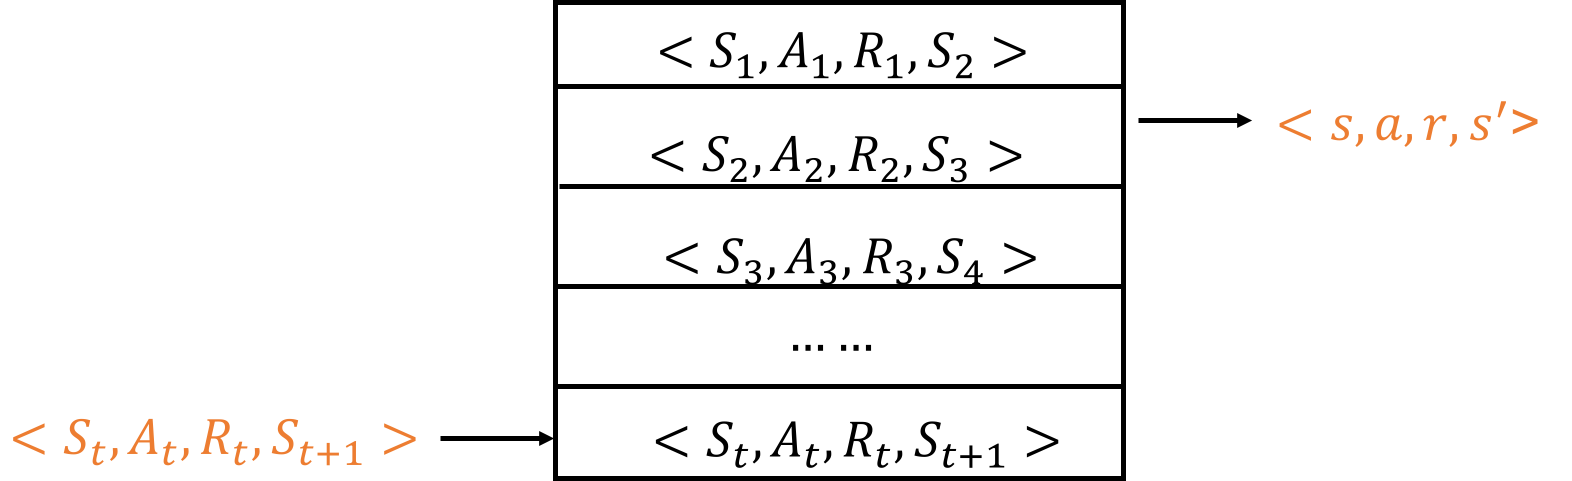
\includegraphics[width=0.85\textwidth]{experience_reply}
\caption{经验回放机制}
\label{fig:experience_reply}
\end{figure}

 \subparagraph{设置独立的目标网络}
使用梯度下降法对参数$\bm{\theta}$进行更新时,可表示为式$\eqref{dituxiajiangq}$:
\begin{equation}\label{dituxiajiangq}
\begin{aligned}
\bm{\theta}_{t+1}=\bm{\theta}_{t}+\alpha[\underbrace{r+\gamma \max_{a^{'}}Q(s^{'},a^{'};\bm{\theta})}_{Target}-Q(s,a;\bm{\theta})]\triangledown Q(s,a;\bm{\theta})
\end{aligned}
\end{equation}

其中,$r+\gamma \max_{a^{'}}Q(s^{'},a^{'};\bm{\theta})$为Q目标值,在计算$\max_{a^{'}}Q(s^{'},a^{'};\bm{\theta})$时用到的参数向量为$\bm{\theta}$。在DQN算法出现之前,利用神经网络逼近值函数时,计算Q目标所用的网络参数向量也是$\bm{\theta}$,与梯度计算$\triangledown Q(s,a;\bm{\theta})$时所使用的参数向量相同,这样就容易导致数据间存在关联性,从而使训练不稳定。

为了解决此问题,DeepMind团队提出使用另一个目标网络(TargetNet)产生Q目标值。具体地,$\bm{\theta}$代表当前网络(MainNet)的输出,用来评估当前状态行为对的值函数;$\bm{\theta}^{-}$代表目标网络的输出,以此求出Q目标值。并且,用于状态行为值函数逼近的网络每一步都要更新,而用于计算目标的网络则是每个固定的步骤更新一次。

因此,值函数的更新变为:
\begin{equation}
\begin{aligned}
\bm{\theta}_{t+1}=\bm{\theta}_{t}+\alpha[\underbrace{r+\gamma \max_{s^{'}}Q(s^{'},a^{'};\bm{\theta}^{-})}_{TargetNet}-\underbrace{Q(s,a;\bm{\theta})]\triangledown Q(s,a;\bm{\theta})}_{MainNet}
\end{aligned}
\end{equation}

\subsection{非参数化函数逼近}
在非参数化函数逼近方法中,参数的个数以及基函数的类型完全由样本来决定,具有很高的灵活性。非参数化函数逼近方法有基于核函数的方法和基于高斯过程的方法。下面以基于核的逼近方法为例进行简单的介绍。

基于核函数的逼近模型可以表示为\eqref{seq2_3_0}:
\begin{equation}\label{seq2_3_0}
\begin{aligned}
&\hat{q}(s,a;\bm{\theta})=\sum^{n}_{i=1}\bm{k}((s,a),(s_{i},a_{i}))\bm{\theta}_{i}\\
&\hat{v}(s;\bm{\theta})=\sum^{n}_{i=1}\bm{k}(s,s_{i})\bm{\theta}_{i}
\end{aligned}
\end{equation}

式$\eqref{seq2_3_0}$中,$\bm{\theta}_{1},\cdots,\bm{\theta}_{n}$为参数向量,$\{(s_{i},a_{i})|i=1,\cdots,n\}$为样本集合,$\bm{k}$为核函数。

非参数化函数逼近过程中完全依赖于样本,虽然带来一定的灵活性,但是其收敛性难以得到保证,而且随着样本规模的扩大,其计算复杂度呈指数级上升。

\section{本章小结}
 本章主要介绍了强化学习中的相关理论知识。首先,对强化学习的整体交互过程进行简单阐述,让读者可以对强化学习有一个直观的认识和体会;接着,介绍了强化学习的形式化框架马尔科夫决策过程以及强化学习的三个基本要素:策略、回报和值函数;然后,总结了强化学习基于模型和模型无关的三种求解方法;最后,针对大规模问题,讨论了求解值函数的三种逼近方法:参数化函数线性逼近、参数化函数非线性逼近以及非参数化函数逼近,为后面章节的开展做了铺垫。
 \cleardoublepage